\title{Project Report - INF560 Calcul Parallèle et Distribuée} %08/fev/2015

\documentclass[12pt,oneside]{article}
\usepackage{amsmath,amssymb,amsthm}
\usepackage[francais]{babel}
\usepackage[utf8]{inputenc}  
\usepackage[T1]{fontenc}
\usepackage{graphicx}
\usepackage{lscape}
\usepackage[hmargin=2.5cm,vmargin=2.5cm,bmargin=2.5cm]{geometry}
\usepackage{caption}
\usepackage{subcaption}
\usepackage{listings}
\usepackage{hyperref}
\usepackage{bbm}
\usepackage{cancel}
\usepackage[official]{eurosym}
\usepackage{pifont}
\usepackage{courier}

\newcommand{\xmark}{\ding{55}}
\newcommand{\select}[2]{\sigma _{#1} \left( #2 \right)}
\newcommand{\project}[2]{\pi _{#1} \left( #2 \right)}
\newcommand{\join}[2]{#1 \bowtie #2}
\newcommand{\rename}[2]{\rho _{#1} \left( #2 \right)}
\newcommand{\agregation}[2]{G _{#1} \left( #2 \right)}

\renewcommand{\thefigure}{\arabic{section}.\arabic{figure}}

\setcounter{secnumdepth}{2}

\begin{document}
\baselineskip=1.5em
\thispagestyle{empty}

\begin{center}
{\Huge \bf Ecole Polytechnique}\\


\vspace{5cm}

{\LARGE{\bf Rapport Final \\ }}
INF560 - Calcul Parallèle et Distribuée

\vspace{6cm}
COELHO LECHNER, Carlos\\
LOBATO GIMENES, Tiago\\
\end{center}

\vspace{5cm}

\begin{center}
\textbf{Palaiseau, France \\  Hiver 2014-2015}
\end{center}


%%%%%%%%%%%%%%%%%%%%%%%%%%%%%%%%%%%%%%%%%%%%%%%%%%
\newpage
\thispagestyle{empty}

\setcounter{tocdepth}{2}
\tableofcontents

\listoffigures

\newpage
\setcounter{page}{1}
%%%%%%%%%%%%%%%%%%%%%%%%%%%%%%%%%%%%%%%%%%%%%%%%%%
\section{Introduction}

Ce rapport provient de nos essais de étudier le problème k-NN(de l'anglais: "\textit{k- nearest neighbors}", en français "\textit{k-plus proches voisins}") dans le cadre du calcul parallèle. Pour cela on a utilisé le langage de programmation CUDA pour les cartes graphiques \textit{NVidia}. Ce problème a plusieurs approches possibles, on en a essayé quelques unes pertinentes au contexte du parallélisme. On montre ici notre approche particulière au problème et on espère que vous trouvez ce problème et les algorithmes utilisés aussi intéressants et amusants que nous les avons trouvé.



%%%%%%%%%%%%%%%%%%%%%%%%%%%%%%%%%%%%%%%%%%%%%%%%%%
\section{Préliminaires}

La méthode des k plus proches voisins est une méthode d’\textit{apprentissage supervisé}.

Dans ce cadre, on dispose d’une base de données d'apprentissage constituée de N couples «entrée-sortie». Pour estimer la sortie associée à une nouvelle entrée x, la méthode consiste à prendre en compte (de façon identique) les k échantillons d'apprentissage dont l’entrée est la plus proche de la nouvelle entrée x, selon une certaine distance.

Par exemple, dans un problème de classification, on retiendra la classe la plus représentée parmi les k sorties associées aux k entrées les plus proches de la nouvelle entrée x.

Ici on regarde le pas d'identification des des k-plus proches voisins d'un point donné et comme on peut optimiser cette étape en utilisant le parallélisme.

\begin{figure}[h]
\centering
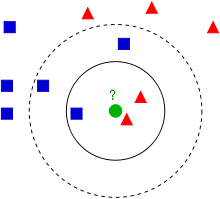
\includegraphics[width=0.3\textwidth]{KNN.png}
\caption{\label{fig:3KNN} Représentation du 3-KNN.}
\end{figure}




%%%%%%%%%%%%%%%%%%%%%%%%%%%%%%%%%%%%%%%%%%%%%%%%%%
\section{Première Solution: Solution CPU - Quicksort}

À titre de comparaison on a fait une solution simple dans la CPU. La solution utilise le sort \texttt{std::sort} de la bibliothèque \texttt{<algorithm>} de C++. Il s'agit d'un tri bien optimisé dont le temps d’exécution attendu(en moyenne) est $O(n.log(n))$. Même si l’implémentation n'est pas spécifiée et varie avec la distribution on peut imaginer pour ce rapport qu'il s'agit d'un quicksort(en français, \textit{tri rapide}).


%%%%%%%%%%%%%%%%%%%%%%%%%%%%%%%%%%%%%%%%%%%%%%%%%%

\section{Deuxième Solution: Parallélisme Naïf}

Notre idée ici était d'utiliser un algorithme parallèle non-optimal tout simplement pour faire une comparaison avec la méthode CPU et pouvoir voir le gain immédiat obtenu par l'utilisation de la carte graphique. Notre première idée était d’implémenter le tri pair-impair mais vu que nous l'avons déjà fait en cours(en Java) nous avons choisi un algorithme diffèrent, le \textit{bitonic sort}(en français, \textit{tri bitonique}). Cet algorithme a un temps d’exécution de $O(n.log^{2}(n))$ mais avec un délai de $O(log^{2}(n))$ (temps parallèle). \newline

 L'astuce du tri bitonique se trouve sur la première figure, extraite de \cite{Venu}.






\begin{figure}[h]
\centering
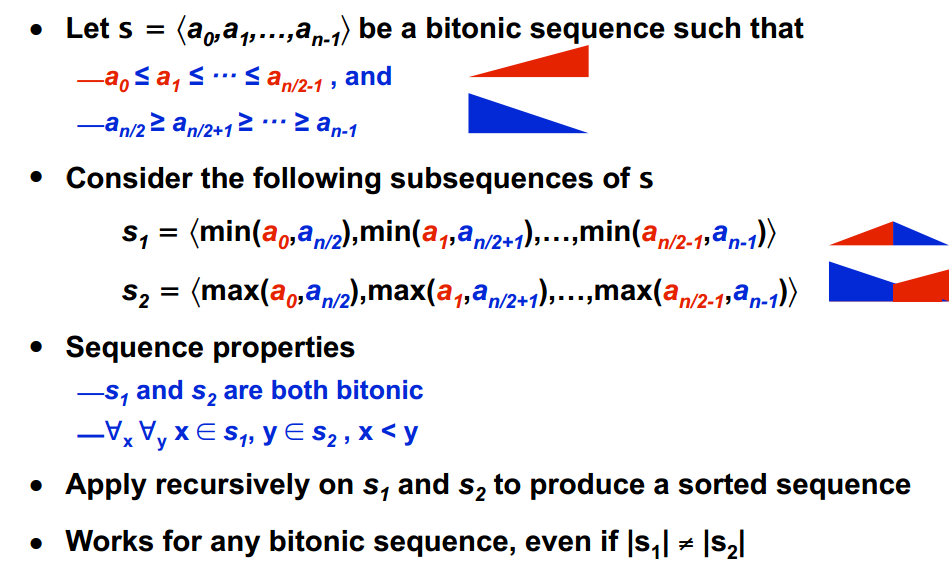
\includegraphics[width=0.5\textwidth]{bitonic_split.png}
\caption{\label{fig:BitonicSort}Représentation de la logique derrière le tri bitonique.}
\end{figure}

\begin{figure}[h]
\centering
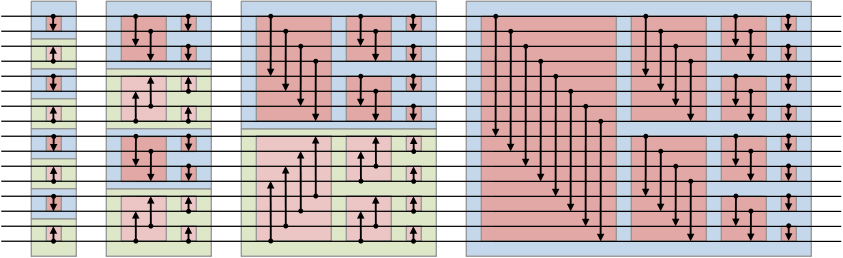
\includegraphics[width=0.6\textwidth]{BitonicSort1.png}
\caption{\label{fig:BitonicSort}Réseau de tri du tri bitonique.}
\end{figure}

\newpage

%%%%%%%%%%%%%%%%%%%%%%%%%%%%%%%%%%%%%%%%%%%%%%%%%%
\section{Troisième Solution: Parallélisme Efficace}

Pour faire une comparaison plus sérieuse on utilise un algorithme bien optimisé pour la GPU: le sort de la bibliothèque \texttt{thrust} de CUDA. On a observé que le gain de performance a été vraiment surprenant dans ce cas.

Pour voir la comparaison entre les 3 méthodes on a fait le graphique suivant:

\begin{figure}[h]
\centering
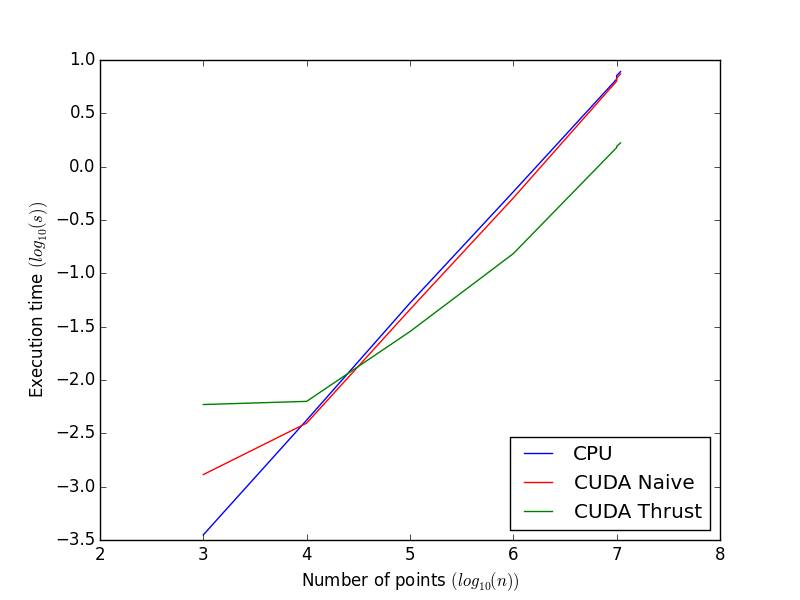
\includegraphics[width=1.0\textwidth]{comparison.jpg}
\caption{\label{fig:Comparaison}Comparaison de temps d'execution sur un \emph{Core i7 4700MQ - GTX850}.}
\end{figure}


%%%%%%%%%%%%%%%%%%%%%%%%%%%%%%%%%%%%%%%%%%%%%%%%%%
\section{Conclusion}

En analysant les résultats, on peut voir que le but initial de solidifier les connaissances du calcul parallèle a été atteint. On a pu avoir le goût du pouvoir de la programmation en GPU.

C'était, surtout, une leçon importante pour nous, aspirants à devenir des ingénieurs logiciels, d'avoir acquis un outil de résolution de problèmes très puissant et très présent dans le monde de l'informatique d'aujourd'hui comme celui de la programmation parallèle. Cela nous offre une nouvelle façon de penser et, donc, ça nous ouvre le champ des possibilités pour l'avenir.

%%%%%%%%%%%%%%%%%%%%%%%%%%%%%%%%%%%%%%%%%%%%%%%%%%
\section{Code}

Les codes complets de nos programmes peuvent être trouvés sur le repositoire GitHub ci-dessous:
  
\url{https://github.com/tlgimenes/CUDAkNN}

%%%%%%%%%%%%%%%%%%%%%%%%%%%%%%%%%%%%%%%%%%%%%%%%%%

\section{Bibliographic References}

  \begin{thebibliography}{1}

  \bibitem{Vazirgiannis} Michalis Vazirgiannis, {\em Notes de cours de "INF582 - BigData: Data Mining} 2015:
  École Polytechnique.
  
  \bibitem{Venu} Sesh Venugopal, {\em Course Notes: Bitonic Sort} 2012: Rutgers University
	\url{http://www.cs.rutgers.edu/~venugopa/parallel_summer2012/bitonic_overview.html}
  
  \bibitem{Lang} H.W. Lang, {\em Course Notes: Bitonic Sort and Sorting Networks} 2010: Fachhochschule Flensburg.
  \url{http://www.iti.fh-flensburg.de/lang/algorithmen/sortieren/bitonic/bitonicen.htm}
  \url{http://www.iti.fh-flensburg.de/lang/algorithmen/sortieren/bitonic/bitonicen.htm}
  
  \bibitem{Lang} E. Goubault, S. Putot, {\em INF560 - Calcul Parallèle et Distribué} 2015: École Polytechnique.
  \url{http://www.enseignement.polytechnique.fr/profs/informatique/Sylvie.Putot/INF560/index.html}
  


  \end{thebibliography}

\end{document}